% !Mode:: "TeX:UTF-8"
%%==========================
%% chapter01.tex for SJTU Master Thesis
%% based on CASthesis
%% modified by wei.jianwen@gmail.com
%% version: 0.3a
%% Encoding: UTF-8
%% last update: Dec 5th, 2010
%%==================================================

%\bibliographystyle{sjtu2} %[此处用于每章都生产参考文献]
\chapter{引言}
\label{chap:intro}

\section{背景和意义}
人体工程学是计算机视觉领域的核心内容,它可以影响到人们方方面面的生活。
例如人脸识别在安全领域的应用,衣服属性分析在衣服搜索领域的应用等等。
这些技术中最基础之一是人体姿势预测。
一般来说,人体姿势预测(HPE)可以应用到很多领域,比如动作识别、图像分割等等。
然而它是一个非常困难的问题,特别是在没有任何辅助信息的情况下,而且对于手臂和腿部等变化比较丰富的人体部位。

众所周知,可以用上下文信息(比如衣服属性、边缘信息等)来解决这个难题。
举例来说,在图\ref{fig:eg}中,a,b,c是三个候选结果,很明显如果我们知道一些上下文信息,很容易判断出只有c是正确解。
因此,这种方法叫做上下文模型,即就是将图片上已知的约束信息加入到HPE问题中,来提高模型的准确性。
近来年,有很多学者做了这方面的工作\cite{deeppose,cvpr09}, 比如\cite{deeppose},他将前背景和后背景对比信息加入到人体姿势预测中。
Ladicky\cite{cvpr09}等人将人体姿势预测与图像分割联系起来,用通过这种联合学习的方式提高HPE的精度。
在Jie Shen\cite{shen2014unified}等人的工作中,他们将人体姿势和衣服属性联合起来进行求解\cite{cvpr09}。

\section{研究内容和方法}
虽然已有的很多工作利用上下文信息提高了人体姿势预测的精度,但是他们都需要进行大量的上下文信息标注才能进行训练,这个非常耗时而且不太实际,对于大数据来说。
在本文中,我们提出了基于隐式衣服属性的人体姿势预测。
我们通过对图画式结构进行扩展来形式化人体姿势预测问题,特别地,我们将衣服属性作为隐变量来建模。
跟传统的基于标注信息进行预测的方法不同,我们不需要显示的标注额外的信息,而且可以高效的进行求解。


在本文中,我们定义了几种比较重要的衣服属性,并且建立了衣服属性和人体部位之间的关系(比如袖子和手臂等)。
进而,我们设计了两种特征,一是人体躯干对应的特征,二是人体躯干和衣服属性的联合特征。
特征是用来刻画问题输入对象的重要参数,所以特征的设计选择直接影响着后续的问题建模与求解。 特征设计是机器学习领域非常重要的问题之一,往往一个问题的特征设计好坏与否直接关系到问题求解的优劣。 HOG特征在前人的很多工作中得到应用,它被证明可以很好的描述物体的形状,因而在我们的工作中,肢干本身的特征采用HOG特征。 关于相邻肢干的联合特征,我们主要考虑两个肢干的相对位置、相对角度和相对距离。
跨问题的特征在于将人体姿势估计和衣服属性识别联系在一起,这也是我们工作的一大创新之处。 这种特征的特点在于,既依赖于一个给定的姿势估计,也依赖于一个给定的衣服属性。 我们通过内积的处理,得到一个由姿势估计和衣服属性同时决定的跨问题特征。

本文采用隐式结构式支持向量机算法来进行模型的训练。
相比于前人的工作,我们是第一个将衣服属性作为隐式变量,然后建立联合模型,对人体姿势估计和衣服属性识别同时进行推导求解的。 如何选择一个正确的模型算法来求解我们的问题是至关重要的,很显然,采用隐式结构式支持向量机来进行参数学习是非常适合我们的问题结构的。 然而结构式的学习框架有很多种,有基于概率模型的,也有基于优化模型的。这里,我们选择使用Chun-Nam等人的包含隐变量的结构式支持向量机(Latent Structural SVM)。 结构式支持向量机的关键在于,它允许研究人员根据自己的问题,设计自己的联合特征和损失函数,接着我们可以根据随机梯度下降法进行目标函数的优化。
所有的隐变量问题都会涉及到隐变量的初始化问题,我们采用$K$-Means聚类算法来初始化隐变量。
接着,我们采用增量迭代的方式来进行参数的学习,即就是最小化隐式结构式支持向量机的目标函数。
更为详尽的,我们采用迭代的方式来训练模型,首先当衣服属性变量确定的时候,我们采用动态规划的算法进行人体姿势的求解。
其次,当人体姿势确定的时候,我们可以采用第三章提出的算法来确定衣服属性的变量。

在以往的工作中,大家对于分别求解两个问题时,都假定问题满足树结构,这样可以使得求解非常高效。 但是现在本文对于两个问题同时建模,破坏了树结构的假设,为此,我们提出了一种迭代求解的算法, 在每一次的迭代过程中,人体的姿势或者衣服的属性都是固定的,从而问题可以规约成一个树模型的求解过程, 使得每一轮的求解可以使用动态规划法进行高效的求解。
在两个公开的数据集上,我们进行了大量的实验,结果显示我们的方法超过了传统最好的方法,并且我们将具有同样衣服属性的照片聚在了一起。

\section{本文的贡献}
总体来说,本文有三大主要贡献:

(1)\textbf{我们提出了一个隐式衣服属性的方法,可以隐性的将衣服属性加入到人体姿势预测问题中。}
通过上述讨论可知,姿势估计和衣服属性识别这两个问题之间有很强的关联性,但是之前的工作,
无论是直接利用姿势估计来进行服饰分析,还是迭代地分割服饰再优化姿势,
或是定义一些能量函数然后通过参数来平衡姿势和服饰的权重,都没有很好地在一个框架下对这两个问题进行统一的建模求解。
在我们的工作中,考虑衣服属性的作用,并且将它作为一个隐式变量,这样就不用手动的去标注衣服属性。

(2)\textbf{我们定义了一些有效的特征来描述人体部位和衣服属性之间的关系。}
特征是用来刻画问题输入对象的重要参数,所以特征的设计选择直接影响着后续的问题建模与求解。 特征设计是机器学习领域非常重要的问题之一,往往一个问题的特征设计好坏与否直接关系到问题求解的优劣。
在我们工作中,人体肢干相关的特征,我们主要考虑两个方面,一是肢干本身的特征,二是相邻肢干的联合特征。 HOG特征在前人的很多工作中得到应用,它被证明可以很好的描述物体的形状,因而在我们的工作中,肢干本身的特征采用HOG特征。 关于相邻肢干的联合特征,我们主要考虑两个肢干的相对位置、相对角度和相对距离。


(3)\textbf{我们提出了一个高效的算法来解决有环图的预测问题(这是一个极其有难度的问题)。}
在以往的工作中,大家对于分别求解两个问题时,都假定问题满足树结构,这样可以使得求解非常高效。 但是现在我们对于两个问题同时建模,破坏了树结构的假设,为此,我们提出了一种迭代求解的算法, 在每一次的迭代过程中,人体的姿势或者衣服的属性都是固定的,从而问题可以规约成一个树模型的求解过程, 使得每一轮的求解可以使用动态规划法进行高效的求解。

\begin{figure}[tbp]
    \centering
    \subfigure[]{
        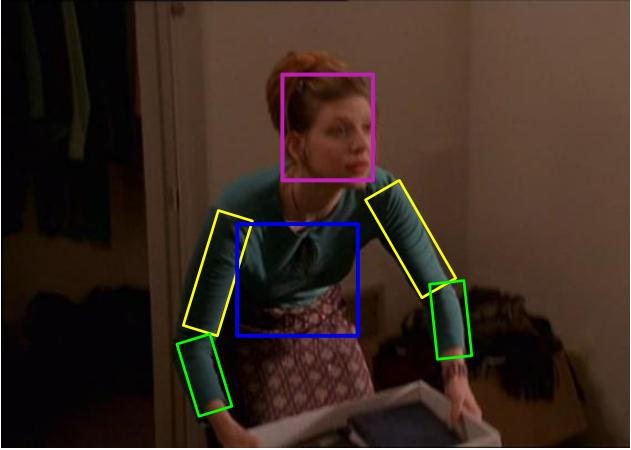
\includegraphics[width=.3\textwidth]{img/eg_a.jpg}
    }
    \subfigure[]{
        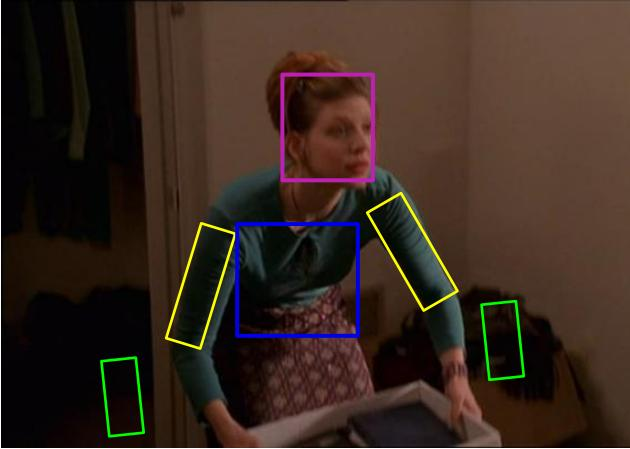
\includegraphics[width=.3\textwidth]{img/eg_b.jpg}
    }
    \subfigure[]{
        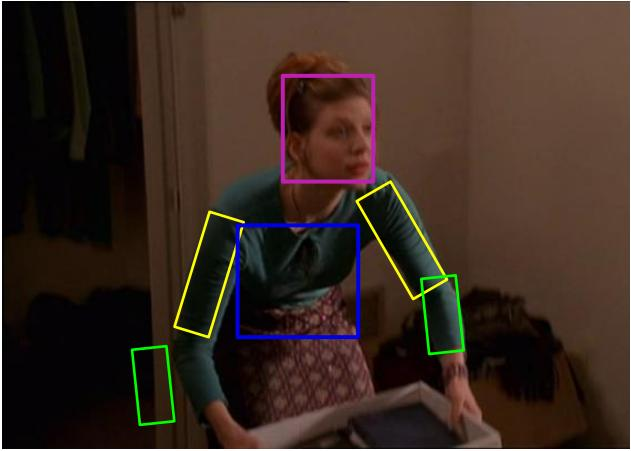
\includegraphics[width=.3\textwidth]{img/eg_c.jpg}
    }
    \bicaption{在人体姿势预测问题中加入衣服属性的动机,
图中所示的三个人体姿势预测的结果,图(b)和图(c)中除了下臂预测错误,其它躯干预测的结果都是正确的。
对于图(c)来说,我们可以通过形状特征来得出左右手臂的不同之处,从而可以将(c)排除掉,
但是在图(b)中,左右手臂的不同之处很微小,我们很难用形状特征来区分出左右手臂。
如果我们知道图中衣服属性的类别值,比如袖子的类别和颜色等。
这样我们就可以根据袖子的颜色或者类别值来区分左右手臂,因为图(b)中左右手臂对应的衣服属性袖子颜色不一致。
最后,我们得到了正确的预测结果,即图(a)。}{在人体姿势预测问题中加入衣服属性的动机
图中所示的三个人体姿势预测的结果,图(b)和图(c)中除了下臂预测错误,其它躯干预测的结果都是正确的。
对于图(c)来说,我们可以通过形状特征来得出左右手臂的不同之处,从而可以将(c)排除掉,
但是在图(b)中,左右手臂的不同之处很微小,我们很难用形状特征来区分出左右手臂。
如果我们知道图中衣服属性的类别值,比如袖子的类别和颜色等。
这样我们就可以根据袖子的颜色或者类别值来区分左右手臂,因为图(b)中左右手臂对应的衣服属性袖子颜色不一致。
最后,我们得到了正确的预测结果,即图(a)。}{Fig}{\textbf{Examples to demonstrate the benefit of integrating clothing attributes into HPE.}
In the three results of HPE, all human poses in (b) and (c) are correct except lower arms.
we can assume that (c) is incorrect based on the great appearance difference between left and right lower arm,
but there is slight appearance difference in (b).
If we know the clothing attribute type, e.g. the sleeve type or color,
we can remove (b) based on the inconsistent color between the upper and lower arms.
Finally, we get the correct estimation (a).}
    \label{fig:eg}
\end{figure}


\section{论文组织}
接下来我们将逐章来介绍我们的工作。
在第二章中,我们介绍了相关的工作,主要分为人体姿势预测(Human Pose Estimation)、衣服属性分析(Clothing Attribute Analysis)、隐变量结构式学习(Structure Learning with Latent Variables)等特定问题领域来介绍。
在第三章中,我们会介绍本文工作的问题背景,主要对本文中涉及到的技术做一个很好的概括。
主要分为图模型(Graphic Model)、图画式结构(Pictorial Structure)、结构式学习(Structure Learning)、形变部位模型(Deformable Part Model)等知识领域来介绍。
在第四章中,我们主要介绍了我们提出的模型和算法,主要分为联合特征设计、模型训练、姿势预测算法等部分来介绍。
第五章我们节选了部分之前跟人体姿势相关的工作来讲述,主要包括基于多媒体数据的事件挖掘(Event Detection)、基于电商平台的衣服搜索(Clothing Search)、基于图片的广告推荐(Advertisement Recommendation)等。
主要阐述人体姿势预测在这些问题上的应用。
在第六章中,我们介绍了实验部分,对数据集、评测指标、实验结果等进行了详细的介绍。
第七章,我们进行了总结,并对未来的工作进行了展望。

\section{本章小结}
本章中,我们简要的介绍了前人在人体姿势识别方面的工作,以及他们的不足,从而提出我们的方法,
克服前人工作的不足支持。
并且我们通过例子说明了加入衣服属性的良好效果。
